%MAGIC COMMANDS
% !TeX TXS-program:compile = txs:///arara
% arara: lualatex: {shell: no, synctex: yes, interaction: batchmode}
% arara: pythontex: {rerun: modified} if exists('pytxcode') && found('pytxcode', 'PYTHONTEX#py')
% arara: lualatex: {shell: no, synctex: yes, interaction: batchmode} if exists('pytxcode') && found('pytxcode', 'PYTHONTEX#py')
% arara: lualatex: {shell: no, synctex: yes, interaction: batchmode} if found('log', '(undefined references|Please rerun|Rerun to get)')

\documentclass[a4paper,11pt]{article}
\usepackage[]{cp-base}
\graphicspath{{./graphics/}}
%variables
\donnees[%
	classe=1\up*{ère} 2M2,
	matiere={[SPÉ.MATHS]},
	mois=Juin,
	typedoc=CAHIER DE VACANCES,
	numdoc=1
]

%formatage
\author{Pierquet}
\title{\nomfichier}
\hypersetup{pdfauthor={Pierquet},pdftitle={\nomfichier},allbordercolors=white,pdfborder=0 0 0,pdfstartview=FitH}
%fancy
\lhead{\entete{\matiere}}
\chead{\entete{\lycee}}
\rhead{\entete{\classe{} - \mois{} \annee}}
\lfoot{\pied{\matiere}}
\cfoot{\logolycee{}}
\rfoot{\pied{\numeropagetot}}
%divers

\begin{document}

%\renewtcolorbox{cexercice}[1][]{%
%	cdefaut,%
%	colframe=MidnightBlue,coltitle=black,colbacktitle=MidnightBlue!15,colback=MidnightBlue!1,
%	title=\large\textcolor{MidnightBlue!50!Black}{\faHubspot}\:\:\textbf{Exercice#1}
%}

\pagestyle{fancy}

\part*{En route vers la Terminale}

\smallskip

\tcbox[sousepreuve,before upper=\faDice\:\:,after upper=\:\:\faChartLine]{\Large  Un \og petit cahier de vacances \fg{}}

\smallskip

\section{Suites et second degré}

\begin{cexercice}[ A1 : calculs des termes de suites]
Calculer les 3 premiers termes de chacune des suites suivantes, en précisant si ces dernières sont définition par récurrence ou de manière explicite :
%
\begin{enumerate}
	\item $u_n = 2n^2-n+1$.
	\item $\begin{dcases} v_1=-2 \\ v_{n+1}=\dfrac{1-v_n}{n} \end{dcases}$.
	\item $w_0=5$ et $w_{n+1}=2w_n-1$.
	\item $t_n=3\big(1+(-1)^n\big)+2$.
\end{enumerate}
\end{cexercice}

\begin{cexercice}[ A2 : suites arithmétiques et géométriques]
\vspace{-0.8\baselineskip}
\begin{enumerate}[leftmargin=*]
	\item Soit $\suiten$ arithmétique de 1\up{er} terme 2 et de raison $-3$.
	\begin{enumerate}
		\item Donner sa définition par formule de récurrence puis sa formule explicite (en fonction de $n$).
		\item En déduire une valeur de $u_{\num{1000}}$.
	\end{enumerate}
	\item Soit $\suiten[v]$ définie pour tout $n$ entier naturel par $v_n = 4 \times 0,5^n$.
	\begin{enumerate}
		\item Expliquer pourquoi cette suite est géométrique.
		\item Donner sa définition par récurrence.
		\item Montrer que la somme $S=v_0+v_2+\ldots+v_{10}$ vaut environ $7,996$.
	\end{enumerate}
\end{enumerate}
\end{cexercice}

\begin{cexercice}[ A3 : « où l’on parle de suite géométrique »]
Une entreprise décide de verser à ses ingénieurs une prime annuelle de 500 euros.

Pour ne pas se dévaluer, il est prévu que chaque année la prime augmente de 2\,\% par rapport à l'année précédente. On
note $\suiten$ la suite des primes avec $u_0 = 500$.
%
\begin{enumerate}
	\item Calculer $u_1$ et $u_2$ (c'est-à-dire la prime versée par l'entreprise la 2\up{ème} année et la 3\up{ème} année).
	\item Exprimer $u_{n+1}$, en fonction de $u_n$. En déduire la nature de la suite $\suiten$.
	\item Déterminer la formule explicite donnant $u_n$ en fonction de $n$.
	\item Déterminer, en détaillant, le sens de variations de la suite $\suiten$.
	\item Un ingénieur compte rester 20 ans dans cette entreprise à partir du moment où est versée la prime.
	\begin{enumerate}
		\item Calculer la prime qu'il touchera la 20\up{ème} année.
		\item Calculer la somme totale $S$ des primes touchées sur les 20 années.
	\end{enumerate}
\end{enumerate}
\end{cexercice}

\begin{cexercice}[ A4 : conjecture de limite à la calculatrice]
À la calculatrice, conjecturer la limite de la suite $\suiten[t]$ définie par $t_0 = 10$ et, pour tout $n \in \N$, $t_{n+1}=0,5t_n-12$.
\end{cexercice}

\pagebreak

\begin{cexercice}[ A5 : monotonie d'une suite\hfill(un peu \og costaud \fg)]
Étudier la monotonie de la suite $\suiten$ définie, pour tout entier naturel non nul $n$, par $u_n = \dfrac{1}{n(n+1)}$ grâce à chacune des trois méthodes suivantes :
%
\begin{enumerate}
	\item en étudiant le signe de la différence $u_{n+1}-u_n$ ;
	\item en comparant le quotient $\dfrac{u_{n+1}}{u_n}$ à $1$ (on s’assurera au préalable que tous les termes de la suite sont strictement positifs) ;
	\item en étudiant les variations de la fonction $f$ telle que $u_n = f\big(u_n\big)$.
\end{enumerate}
\end{cexercice}

\begin{cexercice}[ A6 : résolution d'équations du 2\up{nd} degré]
Résoudre dans $\R$ les équations du second degré suivantes :
\vspace{-0.5\baselineskip}
\begin{multicols}{3}
	\begin{enumerate}
		\item $2x^2-2x-12=0$ ;
		\item $-x^2+x=-2\vphantom{1_{\tfrac11}}$ ;
		\item $3x^2+x\sqrt{12}+1=0$ ;
		\item $4x^2+16=0\vphantom{1_{\tfrac11}}$ ;
		\item $x^2+x=0$ ;
		\item $\big(x^2+5x+6\big)\big(x^2+x+1\big)=0\vphantom{1_{\tfrac11}}$.
	\end{enumerate}
\end{multicols}
\end{cexercice}

\begin{cexercice}[ A7 : signe d’une expression (fonction affine et polynôme du 2\up{nd} degré)]
\vspace{-0.8\baselineskip}
\begin{enumerate}[leftmargin=*]
	\item Déterminer le signe de $4x-7$.
	\item Déterminer le signe de $-2x^2+7x-6$.
\end{enumerate}
\end{cexercice}

\begin{cexercice}[ A8 : résolution d’inéquations du 2\up{nd} degré]
Résoudre, dans $\R$, les inéquations suivantes :
%
\begin{enumerate}
	\item $-x^2+x+2>0$ ;
	\item $3x^2-2x \pp 0$.
\end{enumerate}
\end{cexercice}

\begin{cexercice}[ A9 : une inéquation pour les dominer toutes !\hfill(un peu \og costaud \fg)]
Résoudre, dans $\R$, l'inéquation $\dfrac{2x}{1-x} \pg \dfrac{x+2}{x}$.
\end{cexercice}

\section{Probabilités conditionnelles et variables aléatoires}

\begin{cexercice}[ B1 : maladie et diagnostic]
Des études statistiques montrent que 6\,\% des individus d’une population souffrent d’une maladie donnée.

Un test est utilisé pour diagnostiquer la maladie. On a les résultats statistiques suivants :
\begin{itemize}
	\item sachant qu’un individu est malade, la probabilité qu’il ait un test positif est de $0,95$ ;
	\item sachant qu’un individu n’est pas malade, la probabilité qu’il ait un test négatif est de $0,97$.
\end{itemize}
On désigne par M l’événement « être malade » et par T l’événement « avoir un test positif ».
%
\begin{enumerate}
	\item Représenter la situation à l'aide d'un arbre de probabilités.
	\item Calculer les probabilités des événements $M \cap T$, $\overline{M} \cap \overline{T}$ et $\overline{M} \cap T$.
	\item En déduire la probabilité d’avoir un test positif.
	\item Déterminer la probabilité qu’une personne ayant un test positif soit malade.
\end{enumerate}
\end{cexercice}

\begin{cexercice}[ B2 : probabilité conditionnelle et tableau]
Dans l’étude de certaines maladies, on voudrait savoir si le fait de fumer joue un rôle aggravant ou pas.

On dispose des statistiques ci-contre concernant une population de \num{20000} personnes.
%
\begin{center}
	\begin{tblr}{width=0.8\linewidth,colspec={X[c]X[c]X[c]X[c]},%rows={7mm},
			hline{1}={2-5}{solid,0.8pt},hline{2-5}={solid,0.8pt},
			vline{1}={2-5}{solid,0.8pt},vline{2-5}={solid,0.8pt},
			cell{1}{2,3,4}={lightgray!50},cell{2,3,4}{1}={lightgray!50}
			}
		 & \textbf{Malades} & \textbf{Sains} & \textbf{Total} \\
		\textbf{Fumeurs} & 400 & \num{4600} &  \\
		\textbf{Non-Fumeurs} & 600 & \num{14400} & \\
		\textbf{Total} & & & \\	\end{tblr}
\end{center}
%
On note M l’événement « la personne est malade » et F l’événement « la personne fume ».

On choisit au hasard une personne dans cette population.
%
\begin{enumerate}
	\item Quelle est la probabilité qu’elle soit malade ?
	\item 
	\begin{enumerate}
		\item Calculer $p_F(M)$.
		\item Que représente la probabilité précédente ?
	\end{enumerate}
	\item Si l’on sait que cette personne ne fume pas, quelle est la probabilité qu’elle soit malade ?
	\item Le fait de fumer est-il un facteur aggravant ?
\end{enumerate}
\end{cexercice}

\begin{cexercice}[ B3 : probabilité et temps partiel]
Dans une enquête menée auprès d’une population, on a constaté que :
\begin{itemize}
	\item 60\,\% de la population sont des femmes ;
	\item 56\,\% des femmes travaillent à temps partiel ;
	\item 36\,\% de la population travaillent à temps partiel.
\end{itemize}
%
\begin{enumerate}
	\item Représenter la situation par un arbre pondéré.
	\item On interroge une personne dans la population. Elle affirme qu’elle travaille à temps partiel.
	
	Quelle est la probabilité que cette personne soit un homme ?
\end{enumerate}
\end{cexercice}

\begin{cexercice}[ B4 : loi de probabilité]
La loi de probabilité d’une variable aléatoire $X$ est donnée par le tableau ci-dessous :
%
\begin{center}
	\begin{tblr}{
			hlines={0.8pt},vlines={0.8pt},width=0.8\linewidth,
			colspec={X[2.5,c]X[c]X[c]X[c]X[c]X[c]X[c]X[c]X[c]X[c]},%rows={7mm},
			cell{1,2}{1}={lightgray!50}
		}
		\textbf{Valeurs} $\grasmaths{x_i}$ & 0 & 1 & 2 & 3 & 4 & 5 & 6 & 7 & 8 \\
		$\grasmaths{P(X=x_i)}$ & $0,10$ & $0,05$ & $0,15$ & $0,05$ & $0,10$ & $0,20$ & $0,10$ & $0,10$ & $a$ \\
	\end{tblr}
\end{center}
%
\begin{enumerate}
	\item Déterminer la valeur de $a$.
	\item 
	\begin{enumerate}
		\item Calculer $P(X > 3)$.
		\item Calculer $P(X \pp 3)$.
	\end{enumerate}
\end{enumerate}
\end{cexercice}

\begin{cexercice}[ B5 : variable aléatoire et espérance]
Une urne contient quatre boules numérotées de 1 à 4. On tire au hasard une boule, on note le numéro, on replace cette boule, on tire une deuxième boule et on fait la somme $X$ des nombres inscrits sur les boules.
%
\begin{enumerate}
	\item Déterminer la loi de probabilité de $X$.
	\item Si je gagne une la somme égale à la valeur de $X$, combien puis-je espérer gagner ?
\end{enumerate}
\end{cexercice}

\pagebreak

\begin{cexercice}[ B6 : \og arbre pondéré et variable aléatoire \fg]
Sur la planète Dictat, le gouvernement met en œuvre une politique nataliste.

Toute famille doit avoir au moins un enfant, au plus trois enfants et au plus un garçon.

Dès que l’on a un garçon, on n’a pas d’autre enfant. Soit $X$ la variable aléatoire comptant le nombre d’enfants d’une famille.

On suppose l’équiprobabilité des garçons et des filles à la naissance.
%
\begin{enumerate}
	\item Représenter la situation à l'aide d'un arbre pondéré.
	\item Déterminer la loi de probabilité de $X$.
	\item Calculer $\esp{X}$. Interpréter le résultat.
\end{enumerate}
\end{cexercice}

\section{Fonctions}

\begin{cexercice}[ C1 : lecture de nombres dérivés]
Sur le graphique suivant, $\mathscr{C}_f$ est la courbe représentative d’une fonction $f$ définie sur l’intervalle $\intervFF{-5}{8}$.
%
\begin{center}
	\begin{tikzpicture}[x=0.6cm,y=0.6cm,xmin=-6,xmax=9,xgrille=1,xgrilles=0.5,ymin=-5,ymax=5,ygrille=1,ygrilles=0.5]
		\tgrillep[very thin,gray!50] \axestikz*
		\axextikz[size=\footnotesize]{-5,-4,-3,-2,-1,1,2,3,4,5,6,7,8}
		\axeytikz[size=\footnotesize]{-5,-4,-3,-2,-1,1,2,3,4}
		\draw (0,0) node[below left=2pt] {\footnotesize $0$} ;
		%COURBE
		\def\LISTE{-5/1/1.5§-3/3/0.5§-0.5/3.66/0§2/2/-2§5/-4.55/0§6/-4/1.5§8/2/6}
		\splinetikz[liste=\LISTE,affpoints=false,coeffs=2.5§2.5§2.5§2§2§2,couleur=red]
		%TANGENTES
		\clip (\xmin,\ymin) rectangle (\xmax,\ymax) ;
		\draw[blue,very thick,domain=-5.25:-0.75,samples=2] plot (\x,{0.5*(\x+3)+3}) ;
		\draw[blue,very thick,domain=0.5:3.5,samples=2] plot (\x,{-2*(\x-2)+2}) ;
		\draw[blue,very thick,domain=5:8.5,samples=2] plot (\x,{1.5*(\x-6)-4}) ;
		%LABELS&POINTS
		\filldraw (-5,2) circle[radius=2pt]
				  (-3,3) circle[radius=2pt] node[above] {$A$}
				  (2,2) circle[radius=2pt] node[above right] {$B$}
				  (6,-4) circle[radius=2pt] node[below right] {$C$}
				  (8,-1) circle[radius=2pt] ;
		\draw[blue] (-6,2) node[below right] {$D_1$}
			  (1.5,3) node[above right] {$D_2$}
			  (7,-2.5) node[below right] {$D_3$} ;
		\draw[red] (8,2) node[inner sep=1pt,above right] {$\mathscr{C}_f$} ;
	\end{tikzpicture}
%	
%	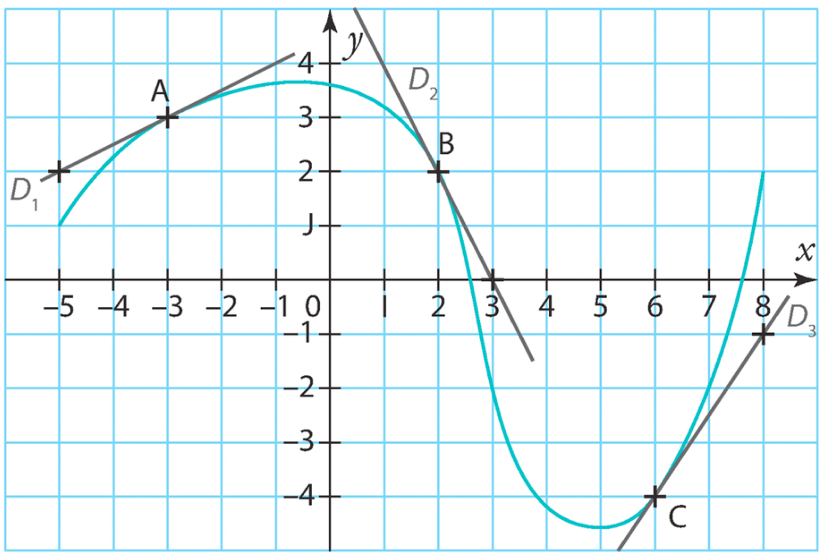
\includegraphics[width=0.5\linewidth]{cdvac_exoc1}
\end{center}
%
${D}_1$, ${D}_2$ et ${D}_3$ sont respectivement les tangentes à $\mathscr{C}_f$ aux points $A$, $B$ et $C$ d’abscisses $-3$, $2$ et $6$.
%
\begin{enumerate}
	\item Lire sur le graphique les valeurs de :
	\begin{enumerate}
		\item $f(-3)$, $f(2)$ et $f(6)$ ;
		\item $f'(-3)$, $f'(2)$ et $f'(6)$.
	\end{enumerate}
	\item 
	\begin{enumerate}
		\item Pour quelle(s) abscisse(s) $a$ semble-t-on avoir $f'(a)=0$ ?
		\item Quelle est la conséquence graphique pour la tangente au point d’abscisse $a$ ?
	\end{enumerate}
\end{enumerate}
\end{cexercice}

\begin{cexercice}[ C2 : dérivées, techniques et dérivation]
Déterminer les fonctions dérivées des fonctions suivantes sur le domaine d’étude précisé :
%
\begin{enumerate}
	\item $f(x)=3x^4-0,5x^2-\dfrac1x$ sur $\mathscr{D}_f = \R^*$.
	\item $g(x)=x\sqrt{x}$ sur $\mathscr{D}_g = \R_{+}^{*}$.
	\item $h(x)=\dfrac{-2x-3}{x+2}$ sur $\mathscr{D}_h = \R \backslash \bigr\{ -2 \bigr\}$.
	\item $i(x)=(1-x)^4$ sur $\mathscr{D}_i = \R$.
\end{enumerate}
\end{cexercice}

\begin{cexercice}[ C3 : nombre dérivé et équation de tangente]
Soit $f$ la fonction définie pour tout réel $x$ par $f(x)=3x^2-2x+1$, on note $\mathscr{C}_f$ sa courbe représentative dans un repère du plan.
%
\begin{enumerate}
	\item 
	\begin{enumerate}
		\item Déterminer $f'(-1)$.
		\item Que représente -- graphiquement -- ce nombre ?
	\end{enumerate}
	\item Déterminer l’équation de la tangente $\mathscr{T}_{-1}$ à $\mathscr{C}_f$ au point d’abscisse $-1$.
\end{enumerate}
\end{cexercice}

\begin{cexercice}[ C4 : étude variations]
Après avoir donné leur ensemble de définition et de dérivabilité, étudier le sens de variation des fonctions suivantes :
%
\begin{enumerate}
	\item $f(x)=-3x^2+2x+1$ ;
	\item $g(x)=\dfrac{1}{3}x^3 - \dfrac14 x^2 - \dfrac{3}{2}x-4$.
\end{enumerate}
\end{cexercice}

\begin{cexercice}[ C5 : utiliser les règles de l'exponentielle]
\vspace{-0.8\baselineskip}
\begin{enumerate}[leftmargin=*]
	\item Simplifier $A=\dfrac{\e^{3x} \times \e^{-x}}{\e^x}$ et $B=\e^x \times \big(\e^{-2x}\big)^3$.
	\item Développer $C=\e^2\left(\e^{-2}+\e\right)$ et $D=\big(\e^4-\e\big)\big(\e^4+\e\big)$.
	\item Factoriser $E=2\e^{6x}-\e^{2x}\vphantom{1_1}$.
\end{enumerate}
\end{cexercice}

\begin{cexercice}[ C6 : dérivées et exponentielle]
Calculer la dérivée des fonctions suivantes sur l’ensemble précisé.
%
\begin{enumerate}
	\item $f(x)=-3\e^x+4\e^{-2x+1}+\e$ sur $\R$.
	\item $g(x)=\big(\e^x+1\big)\big(\e^x-1\big)$ sur $\R$.
	\item $h(x)=\dfrac{4}{\e^{-x}}$ sur $\R$.
	\item $i(x)=\dfrac{\e^x}{x+1}$ sur $\R\backslash\bigr\{ -1 \bigr\}$.
	\item $j(x)=\dfrac{\e^x+1}{\e^x-1}$ sur $\intervOO{0}{+\infty}$.
\end{enumerate}
\end{cexercice}

\begin{cexercice}[ C7 : volume d'une cuve]
On veut construire une cuve métallique à partir d’une plaque carrée de 5~m de côté. À chaque coin de la plaque, on
découpe un carré de côté $x$~m.

En pliant et en soudant, on obtient alors une cuve et on note $\mathscr{V}$ la fonction donnant son volume en fonction des valeurs de $x$.
%
\begin{center}
	\begin{tikzpicture}
		\draw[thick] (0,0) rectangle (5,5) ;
		\def\x{1}
		\def\offset{0.25}
		\draw[thick,fill=lightgray] (0,0) rectangle++ (\x,\x) ;
		\draw[thick,fill=lightgray] (5,0) rectangle++ (-\x,\x) ;
		\draw[thick,fill=lightgray] (0,5) rectangle++ (\x,-\x) ;
		\draw[thick,fill=lightgray] (5,5) rectangle++ (-\x,-\x) ;
		\draw[thick,dashed] (\x,\x) rectangle ({5-\x},{5-\x}) ;
		\draw[very thick,<->,>=stealth'] (0,-\offset) -- (\x,-\offset) node[midway,below] {$x$} ;
		\draw[very thick,<->,>=stealth'] (-\offset,0) -- (-\offset,5) node[midway,left] {$5$} ;
	\end{tikzpicture}
\end{center}
%
\begin{enumerate}
	\item Déterminer l’ensemble de définition puis l’expression de la fonction $\mathscr{V}$ en fonction de $x$.
	\item Étudier les variations de la fonction $\mathscr{V}$.
	\item Déterminer les dimensions de la cuve de volume maximal.
\end{enumerate}
\end{cexercice}

\begin{cexercice}[ C8 : avec une fonction auxiliaire]
Soit $f$ la fonction définie sur $\R$ par $f(x)=(x-2)\e^x + x + 1$.
%
\begin{enumerate}
	\item Déterminer une expression de $f'(x)$.
	\item Soit $g$ la fonction définie sur $\R$ par $g(x) = (x - 1)\e^x + 1$.
	\begin{enumerate}
		\item Étudier les variations de $g$.
		\item En déduire que, pour tout $x \in \R$, $g(x) \pg 0$.
	\end{enumerate}
	\item Montrer que $f'(x)=g(x)$ et en déduire les variations de la fonction $f$ sur $\R$.
\end{enumerate}
\end{cexercice}

\begin{cexercice}[ C9 : un caillou à la mer]
Un enfant monte au sommet d’un phare et laisse tomber verticalement un caillou dans la mer.

On modélise la vitesse (en mètre par seconde) du caillou au bout de $t$ secondes par la fonction : \[ f(t)=6 \times \dfrac{\e^{0,1t}-1}{\e^{0,1t}+1}. \]
\begin{enumerate}
	\item Vérifier que le caillou est bien lâché sans vitesse initiale selon ce modèle.
	\item 
	\begin{enumerate}
		\item Déterminer une expression de $f'(t)$.
		\item Étudier les variations de $f$ sur $\intervFO{0}{+\infty}$.
	\end{enumerate}
	\item La vitesse du caillou dépassera-t-elle les 10 m.s\up{-1} ?
\end{enumerate}
\end{cexercice}

\pagebreak

\section{Géométrie}

\begin{cexercice}[ D1 : savoir utiliser le cercle trigonométrique]
En s'aidant du cercle trigonométrique :
%
\begin{enumerate}[]
	\item Placer $5\pi$ ; $-\dfrac{3\pi}{2}$ ; $\dfrac{7\pi}{3}$ et $-\dfrac{9\pi}{4}$.
	\item Donner la mesure principale de $\dfrac{123\pi}{6}$.
\end{enumerate}
\end{cexercice}

\begin{cexercice}[ D2 : valeurs de cosinus et sinus]
Grâce au cercle trigonométrique, déterminer les valeurs suivantes :
\vspace{-0.5\baselineskip}
\begin{multicols}{3}
	\begin{enumerate}
		\item $\cos\left( \dfrac{3\pi}{4}\right)$ ;
		\item $\cos\left( -\dfrac{\vphantom{1}\pi}{6}\right)$ ;
		\item $\cos\left( \dfrac{9\pi}{2}\right)$ ;
		\item $\cos\left( -\dfrac{11\pi}{3}\right)$ ;
		\item $\cos\left( \dfrac{5\pi}{6}\right)$ ;
		\item $\sin\left( -\dfrac{3\pi}{2}\right)$ ;
		\item $\sin\left( \dfrac{5\pi}{3}\right)$ ;
		\item $\sin\left( -\dfrac{\vphantom{1}\pi}{4}\right)$ ;
		\item $\sin\left( \dfrac{7\pi}{6}\right)$.
	\end{enumerate}
\end{multicols}
\vspace*{0pt}
\end{cexercice}

\begin{cexercice}[ D3 : produit scalaire et vecteurs orthogonaux]
On considère un repère orthonormé du plan.
%
\begin{enumerate}[]
	\item Montrer que $\vect{u} \coordeux{1}{-2}$ et $\vect{v} \coordeux{6}{3}$ sont orthogonaux. Justifier.
	\item $\vect{w} \coordeux{\sqrt{2}}{-1}$ et $\vect{t} \coordeux{2\sqrt{2}}{-4}$ sont-ils orthogonaux ? Justifier.
	\item Déterminer les éventuelles valeurs réelles de $a$ pour que $\vect{t_1} \coordeux{3}{a}$ et $\vect{t_2} \coordeux{6}{-a}$ soient orthogonaux.
\end{enumerate}
\end{cexercice}

\begin{cexercice}[ D4 : droites perpendiculaires et produit scalaire (méthode analytique)]
Dans un repère orthonormé du plan, on donné $A(5\,;\,3)$, $B(8\,;\,-5)$, $C(-1\,;\,0)$ et $D(3\,;\,1,5)$.

Montrer que $(AB)$ et $(CD)$ sont perpendiculaires.
\end{cexercice}

\begin{cexercice}[ D5 : produit scalaire et nature de quadrilatère]
Dans le plan muni d’un repère $\Rij$ orthonormé, on considère les quatre points $A(-3\,;\,2)$ ; $B(-2\,;\,-2)$ ; $C(2\,;\,-1)$ et $D(1\,;\,3)$.
%
\begin{enumerate}[]
	\item Déterminer la valeur de $\vect{AB}\cdot\vect{AD}$.
	\item 
	\begin{enumerate}
		\item Calculer les longueurs $AB$ et $AD$.
		\item Déterminer une valeur de l'angle $\widehat{DAB}$.
	\end{enumerate}
	\item Démontrer que le quadrilatère $ABCD$ est un carré.
\end{enumerate}
\end{cexercice}

\begin{cexercice}[ D6 : équations cartésiennes et vecteur directeur]
\vspace{-0.8\baselineskip}
\begin{enumerate}[leftmargin=*]
	\item Soit $(d)$ la droite passant par $A(4\,;\,2)$ et de vecteur directeur $\vect{u}\coordeux{1}{-3}$. Déterminer une éq. cartésienne de $(d)$.
	\item Soit $(d')$ la droite d’éq. cartésienne $3x - 1,5y + 1 = 0$. Le vecteur $\vect{v} \coordeux{-4,5}{-9}$ est-il un vecteur directeur de $(d')$ ?
\end{enumerate}
\end{cexercice}

\begin{cexercice}[ D7 : droite, vecteurs directeurs et normaux, équations cartésiennes et réduites]
On considère la droite $d$ d’équation réduite $y = -4x + 5$.
%
\begin{enumerate}
	\item Donner un vecteur directeur de $d$.
	\item En déduire un vecteur normal de $d$.
	\item Donner une équation cartésienne de la droite $d'$ perpendiculaire à $d$ passant par le point $A(1\,;\,1)$.
	\item Donner une équation réduite de la droite $d'$.
\end{enumerate}
\end{cexercice}

\begin{cexercice}[ D8 : vecteur normal et équation cartésienne de droite]
\vspace{-0.8\baselineskip}
\begin{enumerate}[leftmargin=*]
	\item Donner un vecteur normal de chacune des droites suivantes :
	\begin{enumerate}
		\item $d_1$ : $-3x + 2y + 1 = 0$ ;
		\item $d_2$ : $5x + y - 6 = 0$ ;
		\item $d_3$ : $y=-2x+4$ ;
		\item $d_4$ : $x=1$.
	\end{enumerate}
	\item Dans chacun des cas, donner une équation cartésienne de la droite passant par $A$ et de vecteur normal $\vect{n}$.
	\begin{enumerate}
		\item $A(4\,;\,1)$ et $\vect{n} \coordeux{1}{-3}$ ;
		\item $A(2\,;\,3)$ et $\vect{n} \coordeux{4}{2}$ ;
		\item $A(-2\,;\,-1)$ et $\vect{n} \coordeux{-3}{-1}$ ;
		\item $A(0\,;\,5)$ et $\vect{n} \coordeux{5}{3}$.
	\end{enumerate}
\end{enumerate}
\end{cexercice}

\begin{cexercice}[ D9 : équation cartésienne de cercle]
\vspace{-0.8\baselineskip}
\begin{enumerate}[leftmargin=*]
	\item Déterminer une équation cartésienne :
	\begin{enumerate}
		\item du cercle de centre $\Omega(5\,;\,4)$ et de rayon $R=2$ ;
		\item du cercle de centre $\Omega(-2\,;\,-3)$ et de rayon $R=5$.
	\end{enumerate}
	\item Dans chacun des cas, donner le centre et le rayon du cercle dont on donne une équation cartésienne :
	\begin{enumerate}
		\item $(x-2)^2+(y+1)^2=25$ ;
		\item $x^2+y^2-4x+5y+3=0$.
	\end{enumerate}
\end{enumerate}
\end{cexercice}

\pagebreak

\section{Algorithmes}

\begin{cexercice}[ E1 : avec un seuil]
On considère la fonction \calgpython{} suivante :

\begin{envcodepythontex}[largeur=8cm,lignes,centre=true]
	def evolu(k):
		u = 200
		n = 0
		while u < k :
			u = 1.2*u + 10
			n = n+1
		return n
\end{envcodepythontex}

Que renvoie l'appel \cpy{evolu(750)} ?
\end{cexercice}

\begin{cexercice}[ E2 : avec une somme]
Soit la suite $\left(u_n\right)$ de premier terme $u_0= 400$ vérifiant la relation, pour tout entier naturel $n$, $u_{n+1} = 0,9u_n +60$.

Compléter la fonction \cpy{Suite} suivante écrite en \calgpython{} qui permet de calculer la somme $S$ des 20 premiers termes de la suite $\left(u_n\right)$.

\begin{envcodepythontex}[largeur=8cm,lignes,centre=true]
	def Suite() :
		S = 0
		U = 400
		for i in range(20) :
			S = ...............
			U = ...............
		return ...
\end{envcodepythontex}
\end{cexercice}

\begin{cexercice}[ E3 : en contexte]
Un apiculteur souhaite étendre son activité de production de miel à une nouvelle région.

Au printemps 2019, il achète $300$ colonies d’abeilles qu’il installe dans cette région.

Il consulte les services spécialisés de la région et s’attend à perdre 8\,\% des colonies chaque hiver. Pour maintenir son activité et la développer, il prévoit d’installer 50 nouvelles colonies chaque printemps, à partir de l’année suivante. On donne le programme suivant écrit en langage \calgpython{} :
\begin{envcodepythontex}[largeur=8cm,lignes,centre=true]
	def algo() :
		C = 300
		N = 0
		while C < 400 :
			C = C*0.92+50
			N = N+1
		return(N)
\end{envcodepythontex}

\begin{enumerate}
	\item Recopier et compléter (en arrondissant à l'entier le plus proche) en ajoutant des colonnes, le tableau ci-dessous qui reproduit l’avancement du programme pas à pas :
	%
	\begin{center}
		\begin{tblr}{hlines,colspec={|Q[c,3cm]|Q[c,2cm]|Q[c,2cm]|Q[c,2cm]|Q[c,2cm]},cells={font=\ttfamily}}
		C 					&300	& 326	& \dotfill 	& \\
		\og C < 400 \fg{} ?	& oui	& oui 	& \dotfill	& \\
	\end{tblr}
	\end{center}
	\item Quelle est la valeur de \cpy{N} renvoyée par le programme ? Interpréter cette valeur dans le contexte de l’exercice.
\end{enumerate}
\end{cexercice}

\pagebreak

\section{Utilisation de la calculatrice}

\begin{cexercice}[ F1 : tracé]
Dans un repère adapté, tracer -- à la calculatrice -- la courbe représentative de la fonction $f$ définie sur $\intervFF{0}{6}$ par $f(x)=(100x+30)\e^{-0,5x}$ .
\end{cexercice}


\begin{cexercice}[ F2 : tracé et outils graphiques, v1]
On considère les fonctions $f(x)=x^3+0,4x^2-8,77x-8,8$ et $g(x)=8x-13$ définies sur $\intervFF{-5}{5}$.
%
\begin{enumerate}
	\item Dans un repère adapté, tracer -- à la calculatrice -- les courbes $\courbe{f}$ et $\courbe{g}$ de manière à obtenir une fenêtre comme ci-dessous :
	\begin{center}
		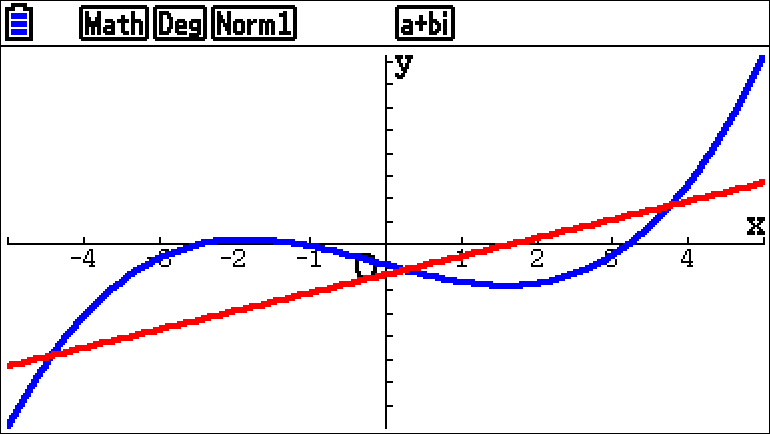
\includegraphics[height=3cm]{tp01_calco_a}
	\end{center}
	\item En utilisant les \ccalg{outils graphiques} de la calculatrice :
	\begin{enumerate}
		\item déterminer les racines de $f$ (autrement dit les solutions de $f(x)=0$) ;
		\item déterminer les solutions de $f(x)=41$ ;
		\item déterminer les solutions de $f(x)=g(x)$.
	\end{enumerate}
\end{enumerate}
\end{cexercice}

\begin{cexercice}[ F3 : tracé et outils graphiques, v2]
On considère les fonctions $f(x)=x\sqrt{36-x^2}$ et $g(x)=x^2-8x+24$ définies sur $\intervFF{0}{6,5}$.
%
\begin{enumerate}
	\item Dans un repère adapté, tracer -- à la calculatrice -- les courbes $\courbe{f}$ et $\courbe{g}$ de manière à obtenir une fenêtre comme ci-dessous :
	\begin{center}
		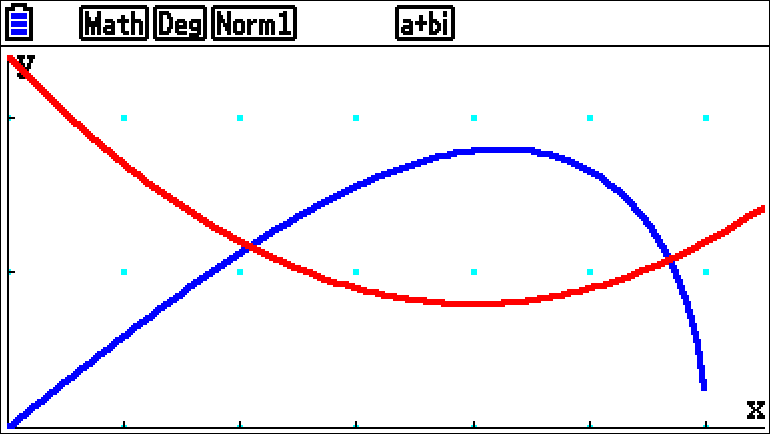
\includegraphics[height=3cm]{tp01_calco_b}
	\end{center}
	\item En utilisant les \ccalg{outils graphiques} de la calculatrice :
	\begin{enumerate}
		\item déterminer le maximum de $f$, ainsi que la valeur de $x$ pour laquelle il est atteint ;
		\item déterminer les solutions de $f(x)=10$ ;
		\item déterminer les solutions de $f(x)=g(x)$ ;
		\item la valeur de $\int_0^5 f(x) \dx$.
	\end{enumerate}
\end{enumerate}
\end{cexercice}

\vfill{}

\hfill{}{\footnotesize \blue \itshape Largement inspiré du travail d'Alexandre Morgan}

\end{document}